\section{Introductie}

Retailbedrijven maken steeds vaker gebruik van IP-camerasystemen voor diefstalpreventie, operationeel beheer en veiligheidsdoeleinden. Ook binnen meubel- en zetelwinkels vormt camerabewaking een vast onderdeel van de dagelijkse werking. In de praktijk worden deze systemen vaak geïntegreerd in het bestaande interne netwerk van de winkel, waarbij netwerksegmentatie en beveiligingsinstellingen beperkt of afwezig zijn. Hierdoor kunnen IP-camera’s een potentieel toegangspunt vormen voor cyberaanvallen of laterale netwerktoegang \parencite{ENISA2024, Naprys2024}.

Deze bachelorproef vertrekt vanuit een concrete casus, namelijk de IP-camerainfrastructuur van meubelzaak De Rore in Deinze. Binnen deze retailomgeving wordt gebruikgemaakt van meerdere IP-cameratypes. Dergelijke heterogene camerainfrastructuren verhogen de complexiteit van configuratie en beheer, wat volgens de literatuur kan leiden tot verhoogde beveiligingsrisico’s wanneer firmwarebeheer, toegangscontrole en netwerkarchitectuur onvoldoende op elkaar zijn afgestemd \parencite{Butun2019}.

De centrale probleemstelling is dat binnen de onderzochte winkelomgeving onvoldoende zicht bestaat op de beveiligingsstatus van het \newline IP-camerasysteem. Het is onduidelijk in welke mate de gebruikte camera’s correct geconfigureerd, actueel gepatcht en veilig geïntegreerd zijn binnen het interne netwerk. Aanwezige kwetsbaarheden kunnen leiden tot ongeautoriseerde toegang tot camerabeelden, manipulatie van instellingen of misbruik van de camerainfrastructuur als toegangspunt tot andere netwerksystemen \parencite{Butun2019}.

Deze bachelorproef richt zich in eerste instantie op de IT-verantwoordelijken en netwerkbeheerders van de meubelzaak die als casus binnen dit onderzoek wordt gebruikt, en focust op het veilig beheren van IP-camerasystemen binnen deze context. Bij uitbreiding zijn de bevindingen en aanbevelingen ook relevant voor \newline IT-verantwoordelijken en netwerkbeheerders binnen andere retail- en KMO-omgevingen die gelijkaardige infrastructuren beheren.

\subsection*{Centrale onderzoeksvraag}

Hoe is de beveiliging van de \newline IP-camerainfrastructuur binnen meubelzaak De Rore ingericht, 
en welke beveiligingsrisico’s zijn daarbij aanwezig?


Vanuit deze centrale vraag worden volgende deelvragen onderzocht:
\begin{itemize}
    \item Welke bekende CVE’s en risico’s bestaan er voor vergelijkbare IP-camera’s?
    \item Hoe communiceert het toestel binnen een retailnetwerk (open poorten, protocollen, standaardinstellingen)?
    \item Kunnen bekende exploits of misconfiguraties effectief worden misbruikt in een gecontroleerde testomgeving?
    \item Welke beveiligingsmaatregelen zijn noodzakelijk om de winkelomgeving beter te beschermen?
\end{itemize}

De doelstelling van dit onderzoek is het opleveren van een onderbouwd beveiligingsadvies voor de onderzochte retailomgeving, 
gebaseerd op een analyse van de bestaande cameraconfiguratie, relevante vakliteratuur en gecontroleerde proof-of-concepttests. 
Daarnaast wordt een gedocumenteerde testopstelling uitgewerkt, zodat de gehanteerde aanpak reproduceerbaar is binnen gelijkaardige retail- en KMO-omgevingen.

\section{State-of-the-art}

De beveiliging van IP-camerasystemen vormt een blijvend aandachtspunt binnen sectoren waarin deze technologie intensief wordt ingezet, zoals de retailsector \parencite{ENISA2024}. In dergelijke omgevingen maken IP-camera’s deel uit van het interne netwerk en worden ze vaak beheerd naast andere kritieke systemen. Uit de literatuur blijkt dat deze apparaten regelmatig kwetsbaarheden vertonen als gevolg van beperkte beveiligingsmechanismen, gebrekkig firmwarebeheer en onveilige standaardconfiguraties \parencite{Butun2019}. Wanneer cameranetwerken onvoldoende gesegmenteerd zijn, kan dit de impact van dergelijke kwetsbaarheden aanzienlijk vergroten.

Onderzoek binnen het domein van IoT-beveiliging toont aan dat IP-camera’s, als embedded systemen, vaak afhankelijk zijn van correcte configuratie door de eindgebruiker \parencite{Butun2019}. Beperkingen in rekenkracht en beveiligingsfunctionaliteit leiden ertoe dat essentiële maatregelen, zoals sterke authenticatie, encryptie van datastromen en adequate toegangscontrole, niet altijd correct worden toegepast \parencite{Butun2019}. Hierdoor kunnen deze toestellen een aantrekkelijk doelwit vormen voor aanvallen die gericht zijn op ongeautoriseerde toegang, misbruik van beheerinterfaces of laterale beweging binnen het netwerk.

Daarnaast wijst zowel academische als professionele literatuur erop dat configuratiefouten in de praktijk frequent voorkomen \parencite{ENISA2024, AlfredCamera2022}. Het niet wijzigen van standaardwachtwoorden, het uitstellen van firmware-updates en het ontbreken van monitoringmechanismen blijven wijdverspreide problemen \parencite{AlfredCamera2022}. In retailomgevingen, waar IT-beheer vaak geen kerntaak is en operationele continuïteit primeert, worden IP-camera’s regelmatig geïntegreerd zonder een expliciete beveiligingsstrategie \parencite{ENISA2024}. Dit verhoogt het risico dat camerainfrastructuren onbedoeld fungeren als toegangspunt tot andere systemen binnen het netwerk.

Hoewel bestaande studies een breed overzicht bieden van kwetsbaarheden en aanvalsvectoren bij IP-camera’s en andere IoT-apparaten, ligt de focus doorgaans op generieke productcategorieën of grootschalige omgevingen \parencite{Butun2019}. Er is minder aandacht voor concrete, heterogene camerainfrastructuren zoals die voorkomen in KMO- en retailcontexten, waar meerdere cameratypes gecombineerd worden binnen één netwerk. Deze bachelorproef positioneert zich binnen dit onderzoeksveld door de beveiliging van een reële IP-camerainfrastructuur in een retailomgeving te analyseren en de vastgestelde risico’s te vertalen naar concrete, contextgebonden aanbevelingen.

\section{Methodologie}

\subsection*{Sprint 1: Contextanalyse en literatuurverankering}

In de eerste sprint wordt een inhoudelijke basis gelegd voor het verdere onderzoek door de IP-camerainfrastructuur van meubelzaak De Rore te analyseren en deze te verankeren in relevante vakliteratuur. De focus ligt niet op het verzamelen van technische kwetsbaarheden, maar op het begrijpen van de context waarin het camerasysteem wordt ingezet en op het identificeren van relevante risico’s die in gelijkaardige omgevingen worden beschreven.

Eerst wordt de bestaande cameraconfiguratie in kaart gebracht op hoofdlijnen. Hierbij wordt aandacht besteed aan het aantal en type camera’s en de plaats van het camerasysteem binnen het interne netwerk. Deze analyse dient om te bepalen welke onderdelen van de infrastructuur beveiligingskritisch zijn en welke aspecten in latere fases verder onderzocht moeten worden.

Parallel hieraan wordt een gerichte literatuurstudie uitgevoerd rond de beveiliging van \newline IP-camerasystemen en IoT-apparaten in KMO- en retailcontexten. Daarbij wordt gefocust op terugkerende probleemcategorieën zoals configuratiefouten, zwakke authenticatie, firmwarebeheer en netwerksegmentatie \parencite{Butun2019}. Gekende kwetsbaarheden en Common Vulnerabilities and Exposures (CVE’s) worden gebruikt als illustratief materiaal om deze probleemcategorieën te duiden, en niet als doel op zich \parencite{CVEdb}.

Op basis van de combinatie van contextanalyse en literatuurstudie wordt een eerste overzicht opgesteld van potentiële beveiligingsrisico’s die relevant zijn voor de onderzochte camerainfrastructuur. Dit overzicht vormt de inhoudelijke input voor de volgende sprints en bepaalt welke onderdelen van de configuratie en het netwerk in detail worden geanalyseerd en getest in een gecontroleerde omgeving.

\subsection*{Sprint 2: Analyse en afbakening}
In deze sprint worden de beveiligingskritische aspecten van de IP-camerainfrastructuur bij meubelzaak De Rore verder geanalyseerd op basis van de bevindingen uit Sprint 1. De focus ligt op het identificeren van relevante configuratie- en netwerkaspecten die volgens de literatuur bijdragen aan verhoogde beveiligingsrisico’s \parencite{Butun2019}. Op basis van deze analyse wordt een onderbouwde afbakening gemaakt van de onderdelen die in een gecontroleerde testomgeving verder onderzocht worden, zodat potentiële kwetsbaarheden veilig en reproduceerbaar kunnen worden aangetoond. Deze sprint bepaalt hiermee de scope voor de daaropvolgende proof-of-conceptfase.

\subsection*{Sprint 3: proof-of-conceptexploitatie en logging}

In de derde sprint worden de belangrijkste kwetsbaarheden uit de CVE-inventaris en de geobserveerde configuratie getest in de labomgeving. De selectie van aanvallen is gebaseerd op literatuur, analyse van de configuratie en contextuele input vanuit de retailomgeving van De Rore, met focus op praktisch relevante scenario’s \parencite{Butun2019}. Aanvallen zoals:
\begin{itemize}
    \item brute-force- of credential-stuffingaanvallen op de webinterface van de camera;
    \item misbruik van onbeschermde of zwak beschermde API-endpoints;
    \item sniffing van videostreams op zoek naar ongeëncrypteerde data;
    \item misbruik van te ruime netwerktoegang (bijvoorbeeld toegang vanaf guest-netwerk).
\end{itemize}

Elke test wordt uitgebreid gelogd:
\begin{itemize}
    \item PCAP-bestanden van het netwerkverkeer;
    \item consolelogs van tools (Nmap, hydra, eigen scripts, \dots);
    \item screenshots van geslaagde en mislukte aanvallen;
    \item eventuele wijzigingen in de configuratie of firmware.
\end{itemize}

De sprint resulteert in een dataset van proof-of-concept-scripts, configuratiebestanden en logbestanden die later gebruikt worden voor analyse en rapportage.

\subsection*{Sprint 4: threat modeling (STRIDE) en mitigatieontwerp}
In de vierde sprint worden de bevindingen uit de voorgaande sprints vertaald naar concrete beveiligingsmaatregelen voor de IP-camerainfrastructuur van meubelzaak De Rore aan de hand van threat modeling op basis van het STRIDE-model \parencite{MicrosoftSTRIDE}. De voorgestelde maatregelen zijn niet gebaseerd op algemene best practices alleen, maar worden expliciet afgeleid uit de vastgestelde risico’s, de geobserveerde configuratie en de context van de onderzochte retailomgeving.

Op basis van de in Sprint 1 geïdentificeerde probleemcategorieën, de in Sprint 2 afgebakende scope en de in Sprint 3 aangetoonde risico’s, worden gerichte aanbevelingen geformuleerd die rekening houden met de operationele realiteit van de winkel. Waar relevant worden deze maatregelen afgestemd op erkende beveiligingsrichtlijnen, zodat ze zowel technisch onderbouwd als praktisch haalbaar zijn binnen een KMO-retailcontext.

Het resultaat van deze sprint bestaat uit een beveiligingsadviesrapport waarin de voorgestelde maatregelen expliciet gekoppeld worden aan de vastgestelde risico’s. Op die manier wordt aangetoond hoe de analyse en proof-of-concepttests hebben bijgedragen aan concrete, contextgebonden aanbevelingen voor het verbeteren van de camerabeveiliging.

\subsection*{Sprint 5: eindrapport en presentatie}

In de laatste sprint worden de resultaten van de voorgaande sprints samengebracht in een eindrapport voor meubelzaak De Rore. Dit rapport bundelt de context en onderzoeksvraag, de geanalyseerde beveiligingsrisico’s en de bevindingen uit de uitgevoerde analyses en gecontroleerde tests. Op basis hiervan wordt een prioriteitenlijst opgesteld en worden gerichte, contextgebonden aanbevelingen geformuleerd.

Daarnaast wordt een presentatie uitgewerkt waarin de belangrijkste bevindingen en voorgestelde maatregelen op een begrijpelijke maar technisch onderbouwde manier worden toegelicht aan de betrokken stakeholders. Ondersteunende technische artefacten die tijdens het onderzoek werden gebruikt, worden gedocumenteerd en beschikbaar gesteld zodat de gevolgde aanpak en vaststellingen traceerbaar blijven.


\begin{figure}[h]
    \centering
    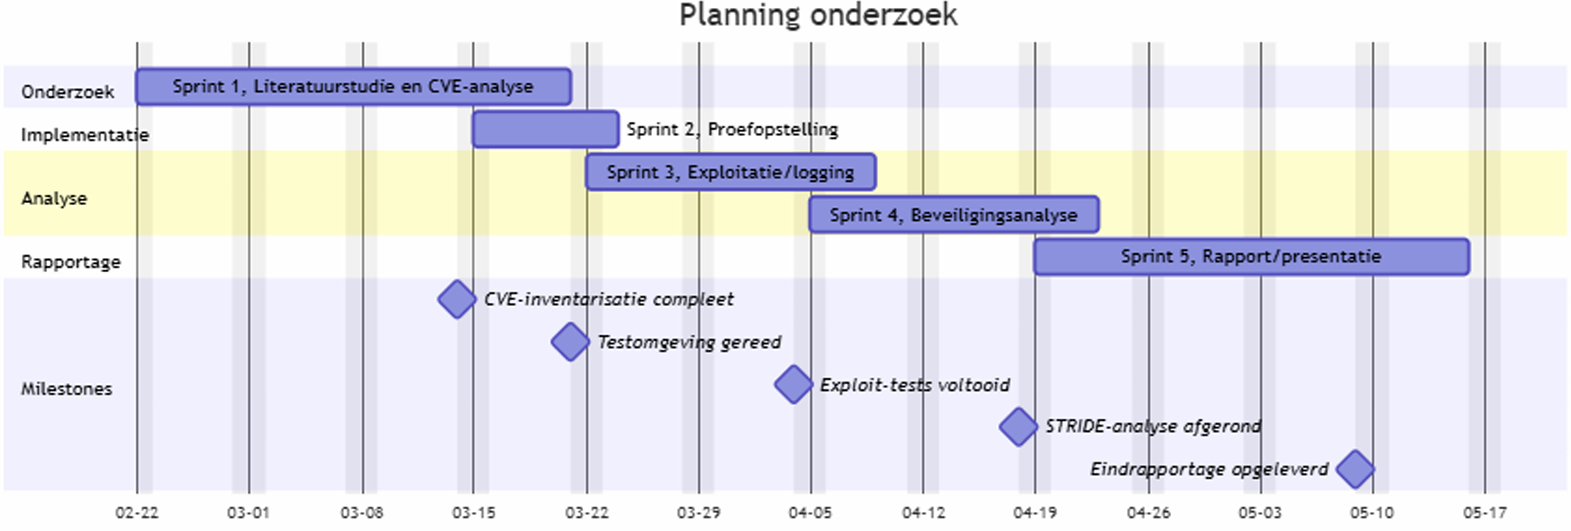
\includegraphics[width=0.55\textwidth]{../voorstel/planning}
    \caption{Planning van het onderzoek met de vijf sprints en milestones.}
    \label{fig:planning-onderzoek}
\end{figure}

\section{Verwachte resultaten en conclusie}

\subsection*{Verwachte resultaten}

Deze bachelorproef beoogt inzicht te verwerven in de beveiligingsstatus van een \newline IP-camerainfrastructuur binnen een concrete retailomgeving. De verwachte resultaten bestaan niet uit vooraf vastgelegde bevindingen, maar uit een onderbouwd overzicht van potentiële beveiligingsrisico’s op basis van literatuurstudie, analyse van de geobserveerde configuratie en gecontroleerde tests. Daarnaast wordt verwacht dat het onderzoek leidt tot een gestructureerd beveiligingsadvies dat afgestemd is op de operationele context van meubelzaak De Rore, evenals tot een gedocumenteerde en reproduceerbare onderzoeksaanpak die ook toepasbaar is binnen gelijkaardige retail- en KMO-omgevingen.

\subsection*{Conclusie}

Dit onderzoeksvoorstel beschrijft een praktijkgericht onderzoek naar de beveiliging van \newline IP-camerasystemen binnen een retailcontext. Door te vertrekken van een concrete casus en door analyse, testopstelling en adviesvorming expliciet op elkaar af te stemmen, wordt beoogd een relevante bijdrage te leveren aan het veilig inzetten van camerabewaking in KMO-omgevingen. De uiteindelijke waarde van het onderzoek ligt in het combineren van technische analyse met contextuele afwegingen, eerder dan in het vooraf vastleggen van specifieke uitkomsten.
